%----------------------------------------------------------------------------------------
%	PACKAGES AND OTHER DOCUMENT CONFIGURATIONS
%----------------------------------------------------------------------------------------

\documentclass{article}

%%%%%%%%%%%%%%%%%%%%%%%%%%%%%%%%%%%%%%%%%
% Lachaise Assignment
% Structure Specification File
% Version 1.0 (26/6/2018)
%
% This template originates from:
% http://www.LaTeXTemplates.com
%
% Authors:
% Marion Lachaise & François Févotte
% Vel (vel@LaTeXTemplates.com)
%
% License:
% CC BY-NC-SA 3.0 (http://creativecommons.org/licenses/by-nc-sa/3.0/)
% 
%%%%%%%%%%%%%%%%%%%%%%%%%%%%%%%%%%%%%%%%%

%----------------------------------------------------------------------------------------
%	PACKAGES AND OTHER DOCUMENT CONFIGURATIONS
%----------------------------------------------------------------------------------------

\usepackage{amsmath,amsfonts,stmaryrd,amssymb} % Math packages

\usepackage{enumerate} % Custom item numbers for enumerations

\usepackage[ruled]{algorithm2e} % Algorithms

\usepackage[framemethod=tikz]{mdframed} % Allows defining custom boxed/framed environments

\usepackage{listings} % File listings, with syntax highlighting
\lstset{
	basicstyle=\ttfamily, % Typeset listings in monospace font
}

%----------------------------------------------------------------------------------------
%	DOCUMENT MARGINS
%----------------------------------------------------------------------------------------

\usepackage{geometry} % Required for adjusting page dimensions and margins

\geometry{
	paper=a4paper, % Paper size, change to letterpaper for US letter size
	top=2.5cm, % Top margin
	bottom=3cm, % Bottom margin
	left=2.5cm, % Left margin
	right=2.5cm, % Right margin
	headheight=14pt, % Header height
	footskip=1.5cm, % Space from the bottom margin to the baseline of the footer
	headsep=1.2cm, % Space from the top margin to the baseline of the header
	%showframe, % Uncomment to show how the type block is set on the page
}

%----------------------------------------------------------------------------------------
%	FONTS
%----------------------------------------------------------------------------------------

\usepackage[utf8]{inputenc} % Required for inputting international characters
\usepackage[T1]{fontenc} % Output font encoding for international characters

\usepackage{XCharter} % Use the XCharter fonts

%----------------------------------------------------------------------------------------
%	COMMAND LINE ENVIRONMENT
%----------------------------------------------------------------------------------------

% Usage:
% \begin{commandline}
%	\begin{verbatim}
%		$ ls
%		
%		Applications	Desktop	...
%	\end{verbatim}
% \end{commandline}

\mdfdefinestyle{commandline}{
	leftmargin=10pt,
	rightmargin=10pt,
	innerleftmargin=15pt,
	middlelinecolor=black!50!white,
	middlelinewidth=2pt,
	frametitlerule=false,
	backgroundcolor=black!5!white,
	frametitle={Command Line},
	frametitlefont={\normalfont\sffamily\color{white}\hspace{-1em}},
	frametitlebackgroundcolor=black!50!white,
	nobreak,
}

% Define a custom environment for command-line snapshots
\newenvironment{commandline}{
	\medskip
	\begin{mdframed}[style=commandline]
}{
	\end{mdframed}
	\medskip
}

%----------------------------------------------------------------------------------------
%	FILE CONTENTS ENVIRONMENT
%----------------------------------------------------------------------------------------

% Usage:
% \begin{file}[optional filename, defaults to "File"]
%	File contents, for example, with a listings environment
% \end{file}

\mdfdefinestyle{file}{
	innertopmargin=1.6\baselineskip,
	innerbottommargin=0.8\baselineskip,
	topline=false, bottomline=false,
	leftline=false, rightline=false,
	leftmargin=2cm,
	rightmargin=2cm,
	singleextra={%
		\draw[fill=black!10!white](P)++(0,-1.2em)rectangle(P-|O);
		\node[anchor=north west]
		at(P-|O){\ttfamily\mdfilename};
		%
		\def\l{3em}
		\draw(O-|P)++(-\l,0)--++(\l,\l)--(P)--(P-|O)--(O)--cycle;
		\draw(O-|P)++(-\l,0)--++(0,\l)--++(\l,0);
	},
	nobreak,
}

% Define a custom environment for file contents
\newenvironment{file}[1][File]{ % Set the default filename to "File"
	\medskip
	\newcommand{\mdfilename}{#1}
	\begin{mdframed}[style=file]
}{
	\end{mdframed}
	\medskip
}

%----------------------------------------------------------------------------------------
%	NUMBERED QUESTIONS ENVIRONMENT
%----------------------------------------------------------------------------------------

% Usage:
% \begin{question}[optional title]
%	Question contents
% \end{question}

\mdfdefinestyle{question}{
	innertopmargin=1.2\baselineskip,
	innerbottommargin=0.8\baselineskip,
	roundcorner=5pt,
	nobreak,
	singleextra={%
		\draw(P-|O)node[xshift=1em,anchor=west,fill=white,draw,rounded corners=5pt]{%
		Question \theQuestion\questionTitle};
	},
}

\newcounter{Question} % Stores the current question number that gets iterated with each new question

% Define a custom environment for numbered questions
\newenvironment{question}[1][\unskip]{
	\bigskip
	\stepcounter{Question}
	\newcommand{\questionTitle}{~#1}
	\begin{mdframed}[style=question]
}{
	\end{mdframed}
	\medskip
}

%----------------------------------------------------------------------------------------
%	WARNING TEXT ENVIRONMENT
%----------------------------------------------------------------------------------------

% Usage:
% \begin{warn}[optional title, defaults to "Warning:"]
%	Contents
% \end{warn}

\mdfdefinestyle{warning}{
	topline=false, bottomline=false,
	leftline=false, rightline=false,
	nobreak,
	singleextra={%
		\draw(P-|O)++(-0.5em,0)node(tmp1){};
		\draw(P-|O)++(0.5em,0)node(tmp2){};
		\fill[black,rotate around={45:(P-|O)}](tmp1)rectangle(tmp2);
		\node at(P-|O){\color{white}\scriptsize\bf !};
		\draw[very thick](P-|O)++(0,-1em)--(O);%--(O-|P);
	}
}

% Define a custom environment for warning text
\newenvironment{warn}[1][Warning:]{ % Set the default warning to "Warning:"
	\medskip
	\begin{mdframed}[style=warning]
		\noindent{\textbf{#1}}
}{
	\end{mdframed}
}

%----------------------------------------------------------------------------------------
%	INFORMATION ENVIRONMENT
%----------------------------------------------------------------------------------------

% Usage:
% \begin{info}[optional title, defaults to "Info:"]
% 	contents
% 	\end{info}

\mdfdefinestyle{info}{%
	topline=false, bottomline=false,
	leftline=false, rightline=false,
	nobreak,
	singleextra={%
		\fill[black](P-|O)circle[radius=0.4em];
		\node at(P-|O){\color{white}\scriptsize\bf i};
		\draw[very thick](P-|O)++(0,-0.8em)--(O);%--(O-|P);
	}
}

% Define a custom environment for information
\newenvironment{info}[1][Info:]{ % Set the default title to "Info:"
	\medskip
	\begin{mdframed}[style=info]
		\noindent{\textbf{#1}}
}{
	\end{mdframed}
}
 % Include the file specifying the document structure and custom commands
\usepackage{graphicx}

%----------------------------------------------------------------------------------------
%	ASSIGNMENT INFORMATION
%----------------------------------------------------------------------------------------

\title{CS221: Project Proposal} % Title of the assignment

\author{	\textbf{Nimisha Tandon}\\  \texttt{nimisha@stanford.edu} \\
		\textbf{Shaila Balaraddi}\\  \texttt{shailaab@stanford.edu} \\ 
		\textbf{Naman Muley}\\      \texttt{ngmuley@stanford.edu}}

\date{\today} % University, school and/or department name(s) and a date

%----------------------------------------------------------------------------------------

\begin{document}

\maketitle % Print the title

%----------------------------------------------------------------------------------------
%	INTRODUCTION
%----------------------------------------------------------------------------------------

\section{Introduction} % Unnumbered section

Identifying information on the internet that could be potentially damaging to a brand is an important function of marketing and PR for a brand. News articles about the entire industry, a product ecosystem or the brand itself, could be relevant to a brand and impact it positively or negatively. A system that provides an impact score by analyzing news and other textual documents can provide useful leads for a brand to get ahead of a PR cycle. For example, articles in Mexican national newspapers about use of guns can be relevant to NRA as a brand in North America and will be helpful for it to shape it's policies.

For the final project we will, first, classify a set of articles into a news groups. Once classified we will analyze the article to produce an impact score for a set of pre-defined parameters. These parameters give insight into how these articles will affect a brand. The impact score can be used to stack rank articles, when presented to the brand.  

\maketitle % Print the title

%----------------------------------------------------------------------------------------
%	SCOPE
%----------------------------------------------------------------------------------------
\section*{Project Scope} % Unnumbered section

This project can be broken down into two stages: a) Classification and b) Impact analysis. Both these operations will deploy ML techniques. The system will take as input some domain data which represents the brand. It will also present to the user certain categories or news groups that the brand is interested in. 

\begin{figure}
	\centering
 	 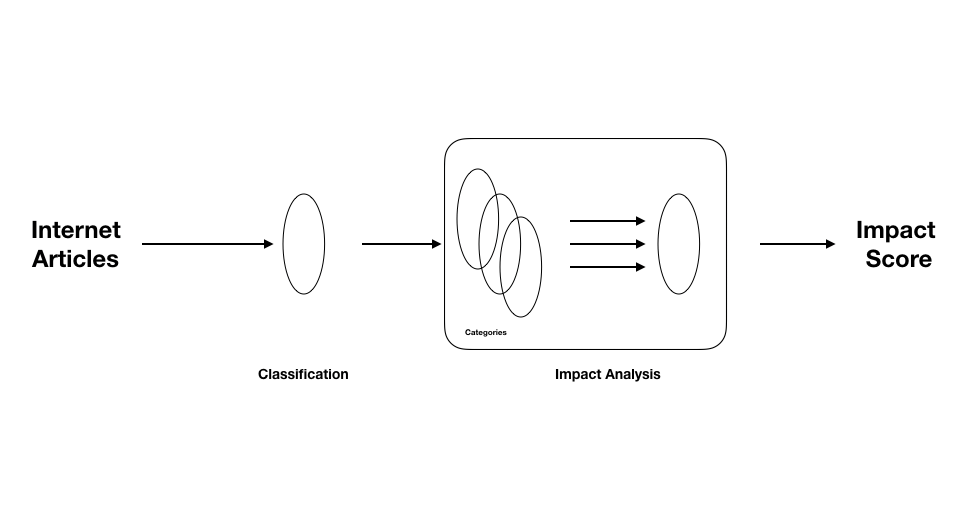
\includegraphics[width=0.6\linewidth]{impact_score.png}
	  \caption{Process Overview}
 	 \label{fig:Impact Potential}
\end{figure}

\subsection{Classification into News Groups}

We will start by building a text classifier. This classifier runs on a recent set of articles provided to it by the application, either siphoned from the internet or gathered from the client. It will then classify these articles into pre-defined categories. 

To build this we will explore multiple techniques like RNN using LSTM, CNN and ML. Based on our findings we plan to either chose one classification model or create an ensemble of the 3 models and use that to classify our article. 

\subsection{Impact Analysis}
Once the article is categorized, providing an impact score based on the classification is the next step. Creating a meaningful impact score is key and part of the challenge. Impact to a brand can be classified based on certain parameters that are important to a brand e.g. market share, sentiment of it's products, sales, research and development etc. Some of these parameters are specific to a category and some others are generally relevant to the brand.

Following are some parameters for a category like \textit{geography}:
\begin{itemize}
	\item \textit{Country}: Is the geographical location talked about in this article one that is highly relevant to the brand?
	\item \textit{Population}: Is this article relevant to a high population number or low?
\end{itemize}

Following are some general parameters that could be relevant to the brand:

\begin{itemize}
	\item \textit{Features}: are people talking about a particular aspect of your product or service?
	\item \textit{Sentiment}: is the article talking about the brand in positive or negative light
	\item \textit{Sales}: is the article talking price, sales or any other monetary factors relevant to the brand
\end{itemize}

%----------------------------------------------------------------------------------------
%	ORACLE AND BASELINE
%----------------------------------------------------------------------------------------

\section{Oracle and Baseline} % Unnumbered section%

We undertook basic exercise to identify upper and lower bounds for our system. These bounds are on the impact score presented to the articles.

\subsection{Oracle}
The Oracle will be a manual classification of articles, and impact score based on the content and its relevance to the subject.
Following is a table of the results of the articles that have any impact to the subject of "guns".

We are interested in articles that reflect a true impact to the brand of guns and NRA.
The following list of articles are categorized and evaluated.

\begin{center}
		\begin{tabular}{ c c c }
			Article Index & Category & Impact Score \\
			55241 & Guns & 0.9 \\ 
			54735 & Guns & 0.8 \\ 
			54606 & Guns & 0.8 \\ 
			54670 & Guns & 0.7 \\ 
			54580 & Guns & 0.7 \\ 
			53294 & Guns & 0.6 \\ 
			54598 & Guns & 0.5 \\ 
			53297 & Guns & 0.5 \\ 
			176846 & Guns & 0.0 \\ 
			54591 & Guns  & 0.0 \\  	 
		\end{tabular}
	\end{center}

As per the Oracle, the scores are dependent on the context of the domain in question.
Hence even though the article 54591 has words like "fire, suicide and survivors", it is an article about an incident, and not about guns.

\subsection{Baseline}
For the baseline we implemented the following:

\begin{enumerate}
	\item \textit{Classifier:} SGD ML classifier, where TF-IDF and vector count was used as features. With this we achieved an accuracy score of 82.4 percent.
	The output of the classifier is what we fed into the impact score analyzer where we tried to rank the documents in terms of their impact score. For calculating the impact score we gave the function a set of words for a given category of the articles. Using these tokens we identified the frequency of these tokens in each of the articles. 

	\item \textit {Impact Analysis:} Given the domain information in the form of some vocabulary, were the set of tokens against which the impact score was being calculated.  However the numbers were not great. We talk about these challenges in the following section
\end{enumerate}

We ran a baseline program for a brand like \textit{guns}. We used the \textit{talk.politics.guns} category already provided in the Newsgroup20 dataset. 

We took as domain input the following vocabulary: \textit{"guns", "shooting", "victim", "mass", "kill", "murder", "weapon", "gun", "nra", "handgun", "assault"}. The baseline performance can be noted down in the following way:

\begin{itemize}
	\item The classifier has 82\% efficiency in classifying the category
	\item The Impact Analysis program resulted into the following Top 10 impact scoring articles. The article indices are indices into the test dataset of articles:
	
	\begin{center}
		\begin{tabular}{ c c }
			Article Index & Impact Score \\
			7274 & 0.05 \\ 
			3613 & 0.03 \\  
			2668 & 0.03 \\ 
			548 & 0.03 \\ 
			1665 & 0.02 \\  
			6763 & 0.02 \\ 
			6896 & 0.02 \\ 
			3781 & 0.01 \\  
			6620 & 0.01 \\ 
			2135 & 0.01 \\ 
		\end{tabular}
	\end{center}
\end{itemize}



\maketitle 
%---------i-------------------------------------------------------------------------------
%	CHALLENGES
%----------------------------------------------------------------------------------------

\section{Challenges} % Unnumbered section

Following are some key challenges facing the project:
\begin{itemize}
	\item \textit{Impact Score:}
	The impact score definition is purposefully kept a bit fluid. The idea of the impact score is to use the category to determine a unique set of characteristics that determine \textit{impactful} texts in that category. In order to improve the impact score we want to explore using the following transformers: 

	\begin{enumerate}
		\item Word2Vec : Using this we would include in the word frequency not just exact words which match but also words that are close in meaning. 
		\item Wordvector averaging 
		\item BERT and ELMO - Since these embedding take into account not just the word but also the context of the input this would help us improve how we calculate the impact score. 
	\end{enumerate}
	
	\item \textit{Category Classifier:} 
	Build a classifier system that can compliment the impact score better. We would also like to improve our classification model for which we want to look at using Neural Network (RNN using LSTM CNN) using Keras and Tensorflow. 
	
	To name a few we would be exploring the below(and more) features to study each ones impact on the classification model. We will compare the output of the model looking at the  Precision , Recall and F1 scores on the validation set: 
	
	\begin{itemize}
		\item Bag of words 
		\item Word2Vec using Glove vectors
		\item TF-IDF
		\item Part of Speech Tagging
		\item Averaging word vectors 
	\end{itemize}

	\item \textit{Dataset:}
	Obtaining the right data set for the training the classifier and impact score system is crucial. Getting the right data to train the classifier on the categories we want to support is a challenge. We have identified the BBC dataset but would like to explore more.
	 
	 Training data for the impact score system is also another challenge. The impact score system will use the category output of the classifier and must also consider the domain in its training. 
	 
\end{itemize}

 
%----------------------------------------------------------------------------------------
%	INFRASTRUCTURE
%----------------------------------------------------------------------------------------

\section{Infrastructure} % Unnumbered section
The details of the infrastructure required for this project is detailed below. The "Application and Interface" section provides a basic information about
the core of the project (Ex: code and any api calls). Compute is used to specify the infrastructure used for the project. The section for "Dataset" will cover
the source, preprocessing and cleanup of data done so far.

\subsection{Application and interfaces}
The project will be written in Python using Scikit-learn library as needed. \newline
The model will accept input from user on the category and will display the outputs as a stack rank of articles on the internet along with their potential impact scores. \newline
This application will interact with the model. \newline
The application will also be responsible for pulling articles from the internet in obtaining test data if required.

\subsection{Compute}
The project will be run on GCP (Google Cloud platform) using the google cloud credits.

\subsection{Dataset}
We will be using the “20 Newsgroup” data set from sklearn. The 20 Newsgroups data set is a collection of approximately 20,000 newsgroup documents, partitioned (nearly) evenly across 20 different newsgroups. \newline
To the best of our knowledge, it was originally collected by Ken Lang, probably for his Newsweeder: Learning to filter netnews paper, though he does not explicitly mention this collection.
The 20 newsgroups collection has become a popular data set for experiments in text applications of machine learning techniques, such as text classification and text clustering. This comes builtin with scikit learn. And can be used directly from there. \newline
We are also looking to use the bbc data set which consists of 2225 documents from the BBC news website corresponding to stories in five topical areas business, entertainment, politics, sport, tech.

The data cleanup and preprocessing is done using the TFIDFVectorizer from Scikit-learn.
We also explored the Bagofwords algorithm before finalizing on the tfidf for training, as this has additional capability of cleaning up words that are too common across documents.
To provide impact analysis, we have manually built a vocabulary set to look for specific domain in the articles, for two categories.


Vocab for medicine
intestine, parasitic, hospital, lungs, ulcer, trauma, accident, illness, chigger, bug, hemorrhage, chronic, patient, clinic, medicine, cancer,health, cholesterol,drug, hdl,ldl, disease
\maketitle % Print the title

%----------------------------------------------------------------------------------------
%	SOCIAL IMPACT
%----------------------------------------------------------------------------------------

\section*{Social Impact} % Unnumbered section
A brand is a financial entity that is interested in knowing potentially impacting content on the internet. Substitute a brand with a social cause like \textit{election}, \textit{poverty}, \textit{amazon rainforest} etc and this system will be able to provide a stack rank of articles that are important to such a cause. 

Also, in the context of fake news, one of the features that the impact analysis system could build is \textit{credibility} where the credibility of a news source is a feature that the impact scoring system takes into account for building an impact score. In that context, this system can be integrated with an RSS feeder plugin which can then recommend potentially impacting articles in a stack rank to people who subscribe to causes like the ones mentioned above.

\end{document}
